\documentclass[letterpaper]{article}
\title{
  IVCalib: A Toolbox to Calibrate Between a Camera and an IMU\\
  \Large{16-831 HW3: Fall 2011}
}
\author{Andrew Chambers, Natasha Kholgade, and Marynel V\'azquez}
\date{}
\usepackage[margin=1in]{geometry}
\usepackage{amsmath}
\usepackage{amssymb}
\usepackage{url}
\usepackage{graphicx}
\usepackage{color}
\usepackage{subfigure}
\usepackage{hyperref}
\newcommand{\bb}[1]{\mathbf{#1}}

\begin{document}

\maketitle

\section{Introduction}

\section{UKF Formulation}
\label{sec:UKF}

In our system, we will ultimately estimate the world space position and orientation of the IMU, $\bb{p}_I^W(t)$ and ${\overline{q}}_I^W(t)$, the velocity of the IMU-camera setup in world space, $\bb{v}^W$, the biases for the gyroscope and accelerometer, $\bb{b}_g(t)$ and $\bb{b}_a(t)$, the gravity vector, $\bb{g}^W(t)$, and, of course, the position and orientation of the camera with respect to the IMU, $\bb{p}_C^I$ and $\overline{q}_C^I$ (i.e. the translation and rotation between the devices). The latter two are the calibration parameters we intend to estimate, and they do not change over time. The state vector, $\bb{x}_s(t)$ has $26 \times 1$ variables.
\begin{equation}
\bb{x}_t=\begin{bmatrix} (\bb{p}_I^W(t))^T & ({\overline{q}}_I^W(t))^T  & (\bb{v}^W)^T  & (\bb{b}_g(t))^T &  (\bb{b}_a(t))^T & (\bb{g}^W(t))^T  & (\bb{p}_C^I)^T & (\overline{q}_C^I)^T\end{bmatrix}
\label{eq:UKF-state}
\end{equation}

The process model uses IMU measurements as control inputs along the vein of Kelly and Sukhatme (ref). The accelerometer and gyroscope biases are modeled as Gaussian random walk processes driven by zero mean noise $\bb{n}_{aw}$ and $\bb{n}_{gw}$, with covariances $\bb{Q}_{aw}$ and $\bb{Q}_{gw}$, while their additive noise is modeled by zero mean noise $\bb{n}_g$ and $\bb{n}_a$, with covariances $\bb{Q}_a$ and $\bb{Q}_g$. The differential equations describing the state evolution are:

\begin{align}
\dot{\bb{p}}_I^W &=\bb{v}^W \nonumber\\ 
\dot{\overline{q}}_I^W&=\frac{1}{2}\begin{bmatrix}0 & -(\omega^I)^T \\ \omega^I & -[ \omega^I ]_{\times} \end{bmatrix}  \nonumber\\
\dot{\bb{v}}^W &=\bb{a}^W  \nonumber\\
\dot{\bb{g}}^W &=\bb{0}_{3 \times 1}  \nonumber\\
\dot{\bb{b}}_g&=\bb{n}_{gw}  \nonumber\\
\dot{\bb{b}}_a&=\bb{n}_{aw}  \nonumber\\
\dot{\bb{p}}_C^I&=\bb{0}_{3 \times 1} \nonumber\\
\dot{\overline{q}}_C^I&=\bb{0}_{4 \times 1}
\end{align}

The measured acceleration and gravity are given as
\begin{align}
\omega_m&=\omega^I+\bb{b}_g+\bb{n}_g \nonumber \\
\bb{a}_m&=\bb{C}^T(\overline{q}_I^W)(\bb{a}^W-\bb{g}^W)+\bb{b}_a+\bb{n}_a
\end{align}

The entire process noise mean and covariance are

\begin{align}
\bb{n}=\begin{bmatrix} \bb{n}_{gw} \\ \bb{n}_{aw} \\ \bb{n}_g\\ \bb{n}_a \end{bmatrix}, \bb{Q}=\begin{bmatrix} \bb{Q}_{gw} & & & \\ & \bb{Q}_{aw} & & \\ & & \bb{Q}_g & \\ & & & \bb{Q}_a \end{bmatrix}
\end{align}

During measurement, the camera images the world points, $\bb{p}_{l_i}^W$ (which in our current system, we assume are known). To take the world points from the world coordinate system to the camera's coordinate system $\bb{p}_{l_i}^C$, we apply the rotation and orientation of the IMU in the world coordinate system, and those of the camera with respect to the IMU:

\begin{align}
\bb{p}_{l_i}^C=(\bb{C}(\overline{q}_C^I))^T \left((\bb{C}(\overline{q}_I^W))^T \left(\bb{p}_{l_i}^W-\bb{p}_I^W\right) -\bb{p}_C^I \right)
\end{align}

We model the projected points $u_i$ and $v_i$ in the camera's coordinate system with additive measurement noise. 

\begin{align}
\bb{z}_i=\begin{bmatrix} u_i \\ v_i \end{bmatrix}&=\begin{bmatrix} x_i' \\ y_i' \end{bmatrix}+\eta_i \nonumber\\
\begin{bmatrix} x_i' \\ y_i' \\ 1 \end{bmatrix} & \equiv K\begin{bmatrix} x_i \\ y_i  \\ z_i \end{bmatrix}
\end{align}



\section{Tests}

We decided to implement the filter progressively given the complexity
of the state space. We considered a reduced number of unknowns and a
very simple model at the beginning. The following subsections detail
our progress towards a complete toolbox for sensor-to-sensor
calibration.

\subsection{Estimating rigid body translation}

Our first simulation test consisted on effectively estimating the
position in 3D space of the rigid body sensor suite. We assumed our
inertial sensor was able to give us velocity instead of acceleration,
and that the body did not rotate throughout the simulation. No bias
or gravity were considered in the model.

We generated a path for the sensor suite with constant linear
velocity, and altered ground truth velocity with zero-mean Gaussian
noise. Our state vector had a dimensionality of $3$ in this test,
instead of $26$ as in (\ref{eq:UKF-state}). The process noise
covariance was a $3 \times 3$ diagonal matrix.
\begin{equation}
\bb{x}_t=\begin{bmatrix} p_{I_x}^W(t) & p_{I_y}^W(t) & p_{I_z}^W(t) \end{bmatrix} 
\hspace{4em}
Q = \begin{bmatrix} 
\sigma_x^2 & 0 & 0\\ 
0 & \sigma_y^2 & 0\\ 
0 & 0 & \sigma_z^2
\end{bmatrix} 
\label{eq:TranslationTest-stateVec}
\end{equation}

We automatically generated landmarks by uniformly sampling 3D points
in our simulated world, and projected them into our simulated camera
sensor. Figure \ref{fig:TranslationTest-uniformPoints} depicts a
possible distribution of landmarks in our simulated world.

% TODO. Might be a good idea to regenerate this picture with whatever
% point distribution we used before submitting the report..
\begin{figure}[h!tbp]
\centering
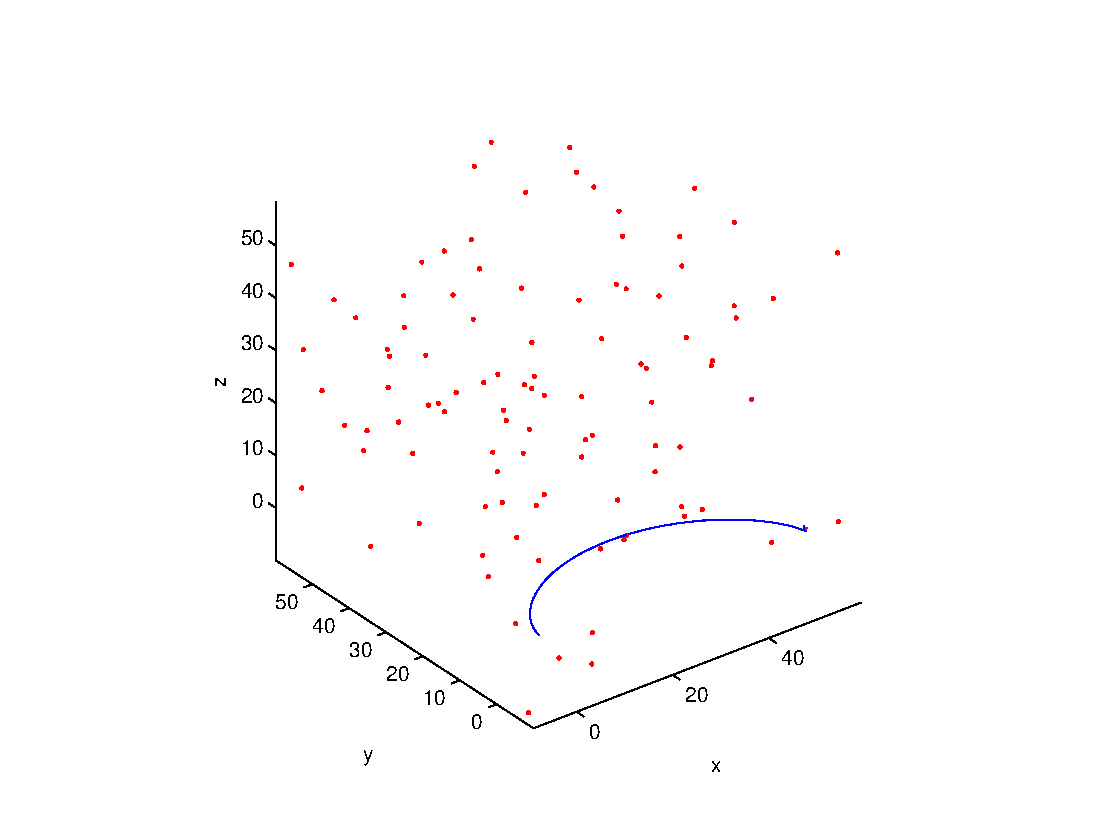
\includegraphics[width=0.5\linewidth]{uniform_points}
\caption{Automatically generated landmarks (red points) in our simulated
  world. The blue line depicts the uniform velocity path used for the
  rigid body translation test.}
\label{fig:TranslationTest-uniformPoints}
\end{figure}

\section{Future work}

% References (working on bib file)

\end{document}

